\section{Representing An Artist's Life}\label{sec:representing-artists-life}
If we think about how the artist’s life is presented to the public, we first speak of biography books and memoirs~\citep{isaacson2017leonardo,
    tomkins1999duchamp, herrera1983frida}, then museum exhibitions, articles and interviews, and others. Essentially, it is mostly a sort of
written form and in some cases includes visual aspects, like in exhibitions.

\begin{figure}[h!]
    \begin{center}
        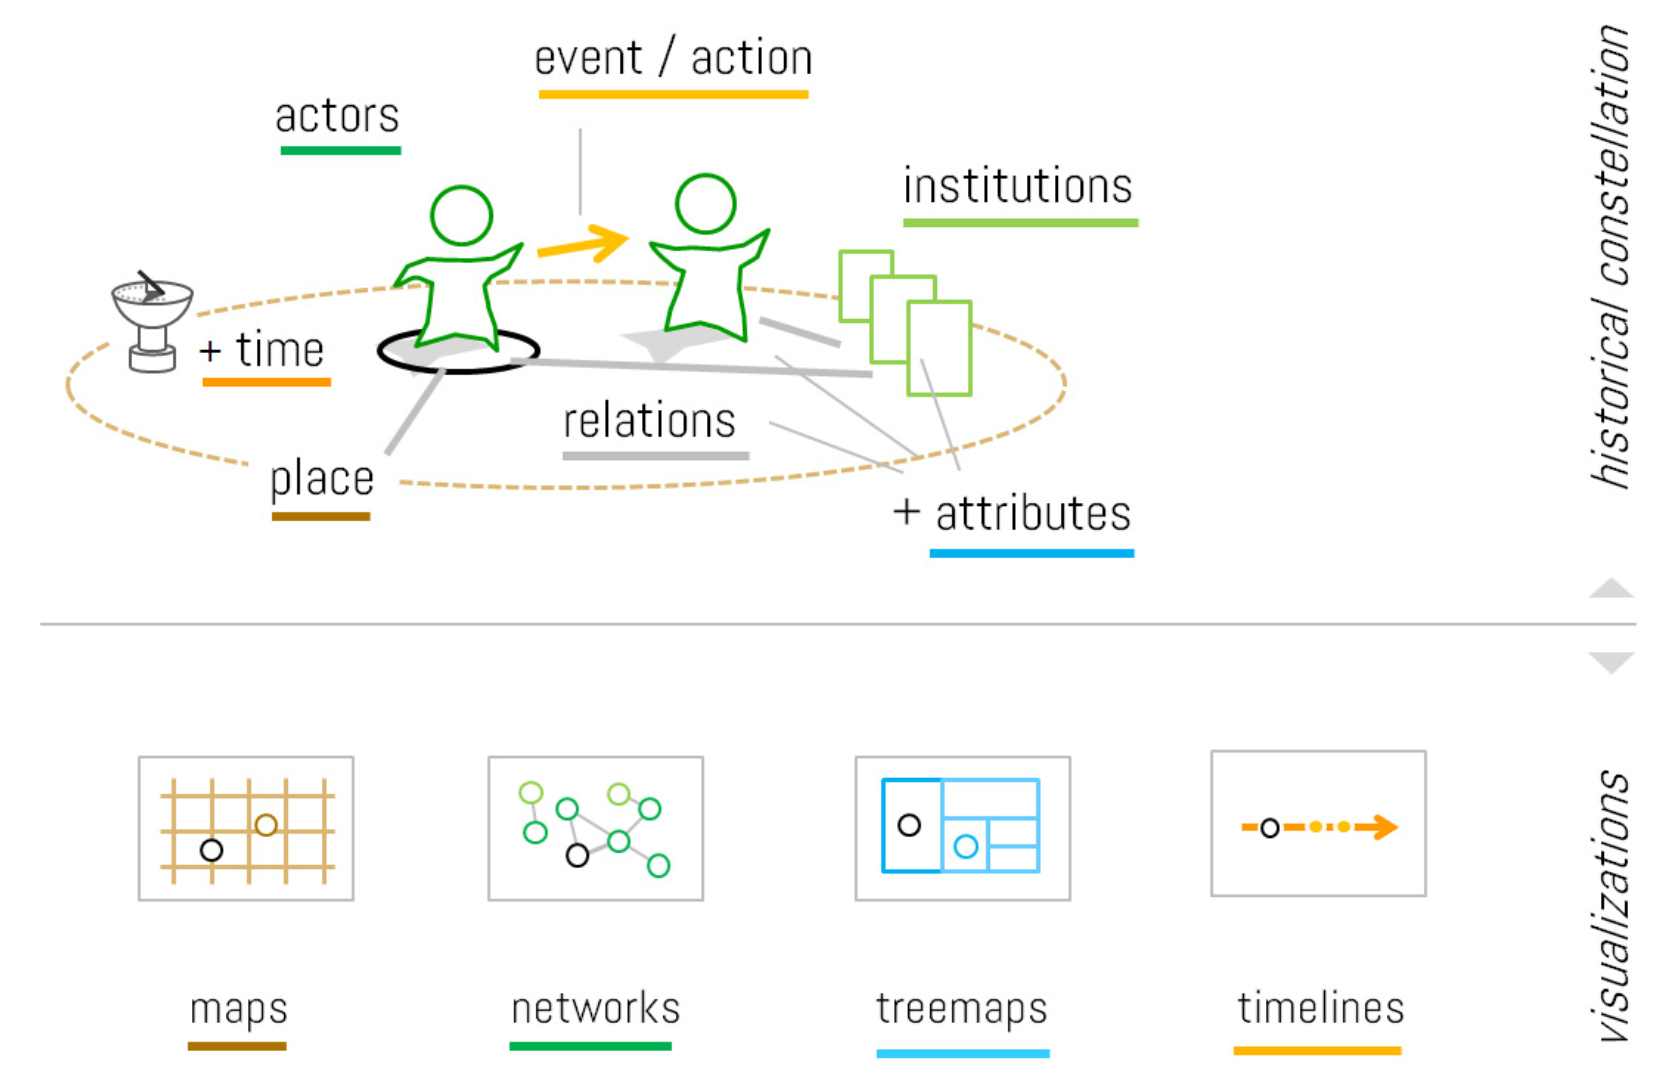
\includegraphics[width=0.9\textwidth]{graphics/2-literature-review/22}
    \end{center}
    \caption{Biographical investigation of an individual and some usual types of visualizations~\citep{windhager2017synoptic}}
    \label{fig:figure2.22}
\end{figure}

The study of biographies has been a usual and important investigative perspective for centuries~\citep{windhager2017synoptic}. The paper also
states that biographical data is usually
\begin{enumerate}
    \item \emph{multidimensional} -- has spatial, relational, and categorical dimensions, and all of these are commonly.
    \item \emph{time-oriented} -- entities are linked to events or connected to timestamps.
\end{enumerate}

According to these properties of biographical data, we can see that the space-time cube is the suitable choice for our case. We have a
spatial dimension, as well as a relational dimension, and both of them are linked to the events in the artist’s life.

Mayr and Windhager~\citep{mayr2018once} list some common hybrid visualizations of spatial (brown) and temporal (orange) data dimensions,
including the space-time cube: a) multiple coordinated views, b) animation/slideshow, c) color-coded layer superimposition, d) layer
juxtaposition, e) space-time cube.

\begin{figure}[hbt!]
    \begin{center}
        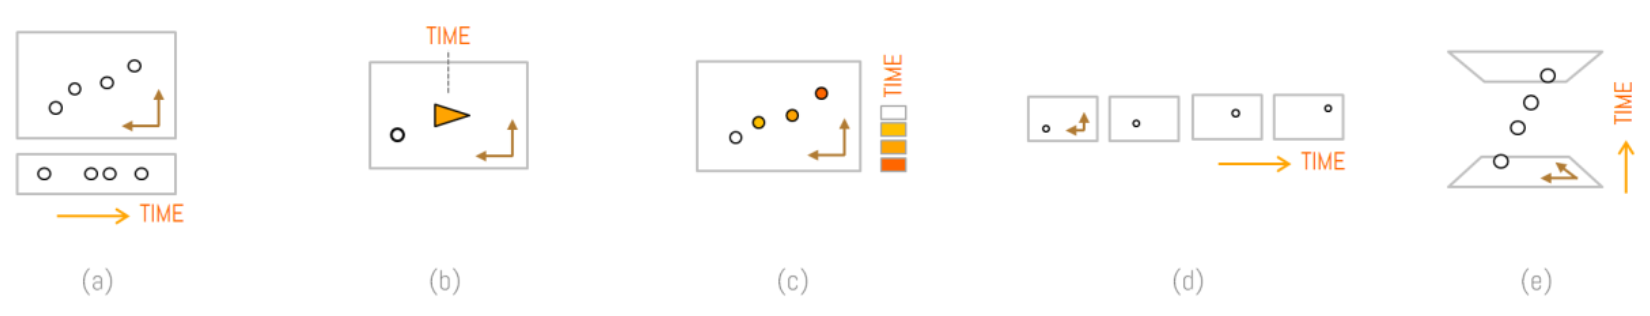
\includegraphics[width=\textwidth]{graphics/2-literature-review/23}
    \end{center}
    \caption{Hybrid visualizations for spatial and temporal data dimensions}
    \label{fig:figure2.23}
\end{figure}

Usually, one-dimensional visualizations like maps and timelines only allow the analysis of single data dimensions and there is no space for
the examination of cross-dimensions. These hybrid visualizations can provide a visual comparison and combination of biographical patterns that
include the similarities and differences among several artists~\citep{windhager2017beyond}.

Capturing the essence of artists’ life furthermore depends on what we want to present. Is it related to their work only or do we include other
parameters as well - family connections, places they lived in, relations to other artists, or some others? Fitting such things as full knowledge of
an artist’s life into a few written pages or simple visualizations is a hard task to do. It is necessary to extract the most important aspects and
capture them in the best possible way. We will seek to do this in the implementation part of this thesis altering the previously seen space-time
cube. But before doing that, we need to present some already-seen visualizations associated with artists and their lives.

The first visualization is an anthology of ten painters’ lives by Giorgia Lupi and Michela Buttignol~\citep{lupi_buttignol}. They used
pictorial elements related to artists’ styles to present their lives visually. Each artist was presented with a timeline composed of the life
events and artworks using colors and shapes associated with their style. The example shown in \Cref{fig:figure2.24} is the life of Picasso.

\begin{figure}[hbt!]
    \begin{center}
        \includegraphics[width=1.3\textwidth, angle=90]{graphics/2-literature-review/24}
    \end{center}
    \caption{Pictorial representation of Picasso's life}
    \label{fig:figure2.24}
\end{figure}

\clearpage

We can see the timeline of the artist from his birthdate and birthplace to his death. Above the line are his love affair relationships with
some of them ending in marriage. This part also presents places he traveled to, his siblings, and his offspring, each colored
differently. Everything related to their personal life is shown in the upper part. The lower part is concerned with their artistic world. We
can spot the distinctive artistic periods and amount of works during that time, acquaintances, awards, and events. The most important part of
the visualization is the artworks where the painter’s masterpieces are presented in small shapes and colored according to the artwork’s
palette. All of them are also grouped according to the subject of the work. The pictogram’s size depends on the real painting size and is
divided into three categories: small, medium, and large. The visualization covers a lot of things related to the artist’s life, but everything
is explained thoroughly.

The second example is an interactive timeline of Andrew Wyeth’s life shown in the figure below~\citep{wyeth_2021}.

\begin{figure}[hbt!]
    \begin{center}
        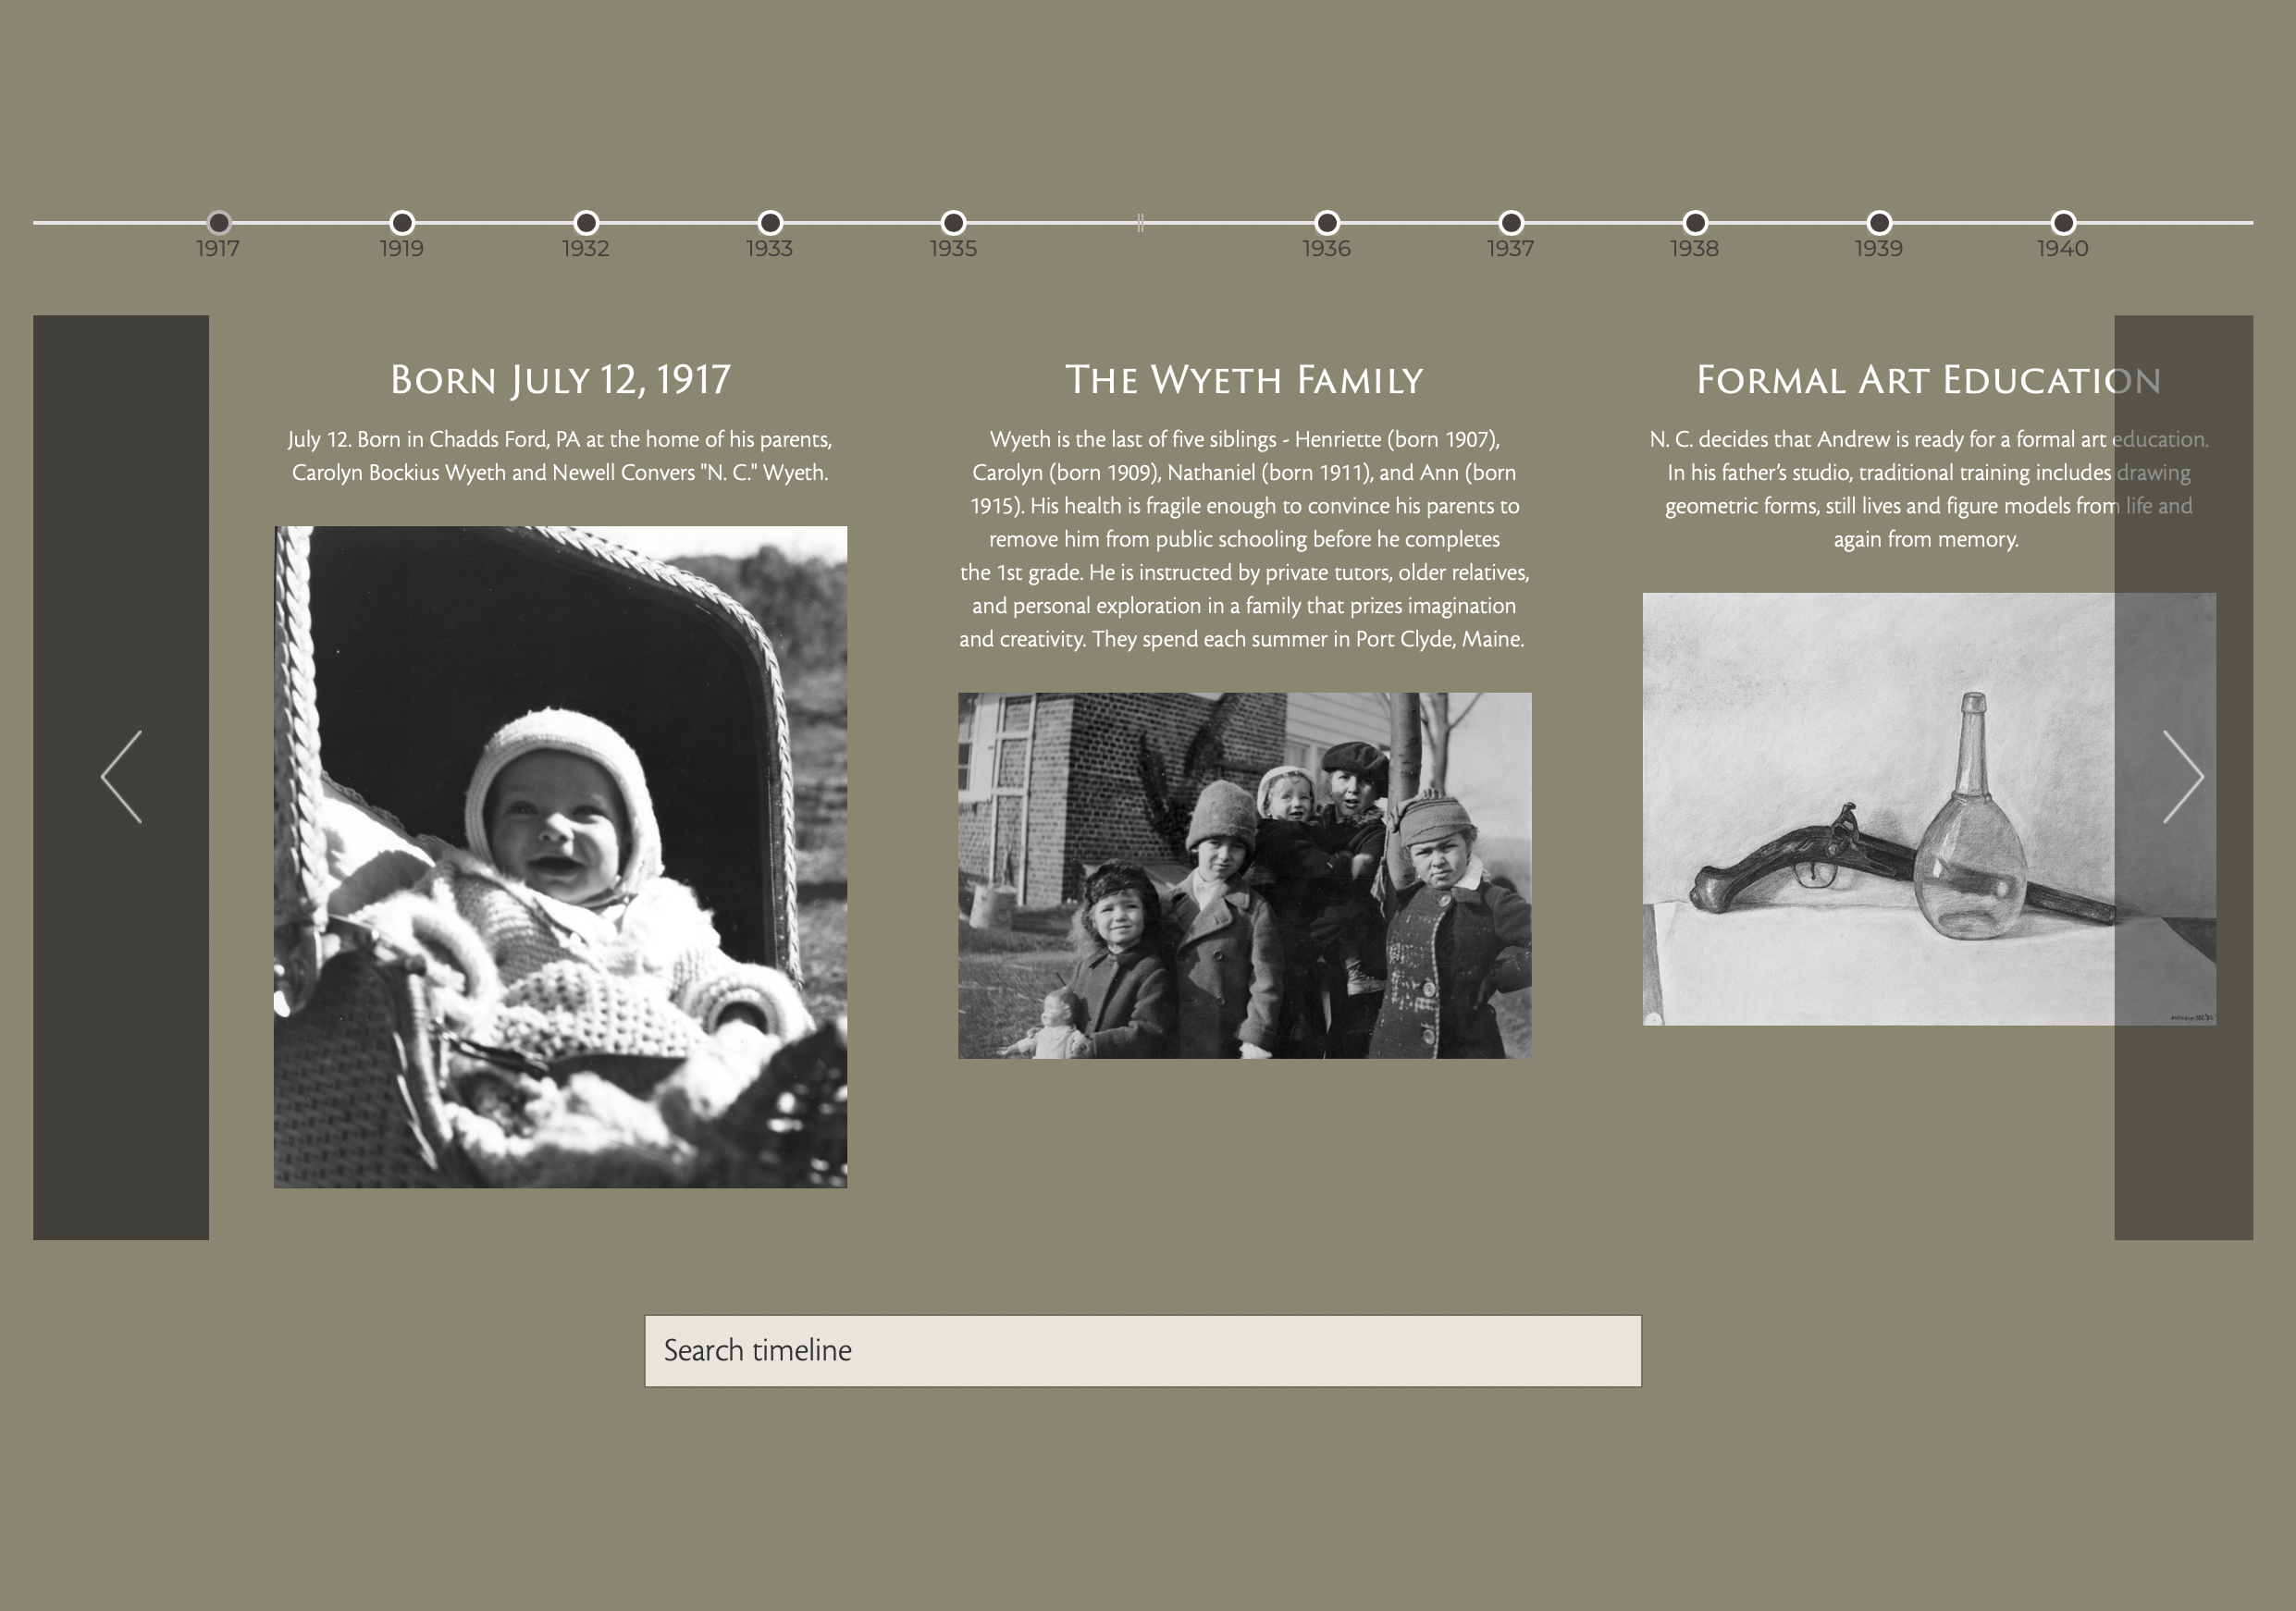
\includegraphics[width=0.9\textwidth]{graphics/2-literature-review/25}
    \end{center}
    \caption{Andrew Wyeth’s life timeline}
    \label{fig:figure2.25}
\end{figure}

The left and right arrows allow the exploration of his life with the year indicators at the top. It is possible to skip to a certain year and
explore only that part. At the bottom, there is a search box for searching the timeline and showing only those events that contain a searched
term.\footnote{You can explore Andrew Wyeth's timeline at \url{https://andrewwyeth.com/timeline/}}

We have seen from the first two examples that they used the timeline to present the artist’s life. Drawing a straight line and arranging
life events, relationships, artworks, and everything else seems like an engaging way of capturing one’s life. The first example elevated the
conventional timeline and introduced innovative ways of showing all the details about the artist’s life. Although the visualization was
two-dimensional and not interactive, it was still an attractive solution. The second example was a typical timeline with photos and written
captions included. On the other hand, it had an interactive aspect which contributed to easier maneuvering and finding information of interest
faster.

\begin{figure}[hbt!]
    \begin{center}
        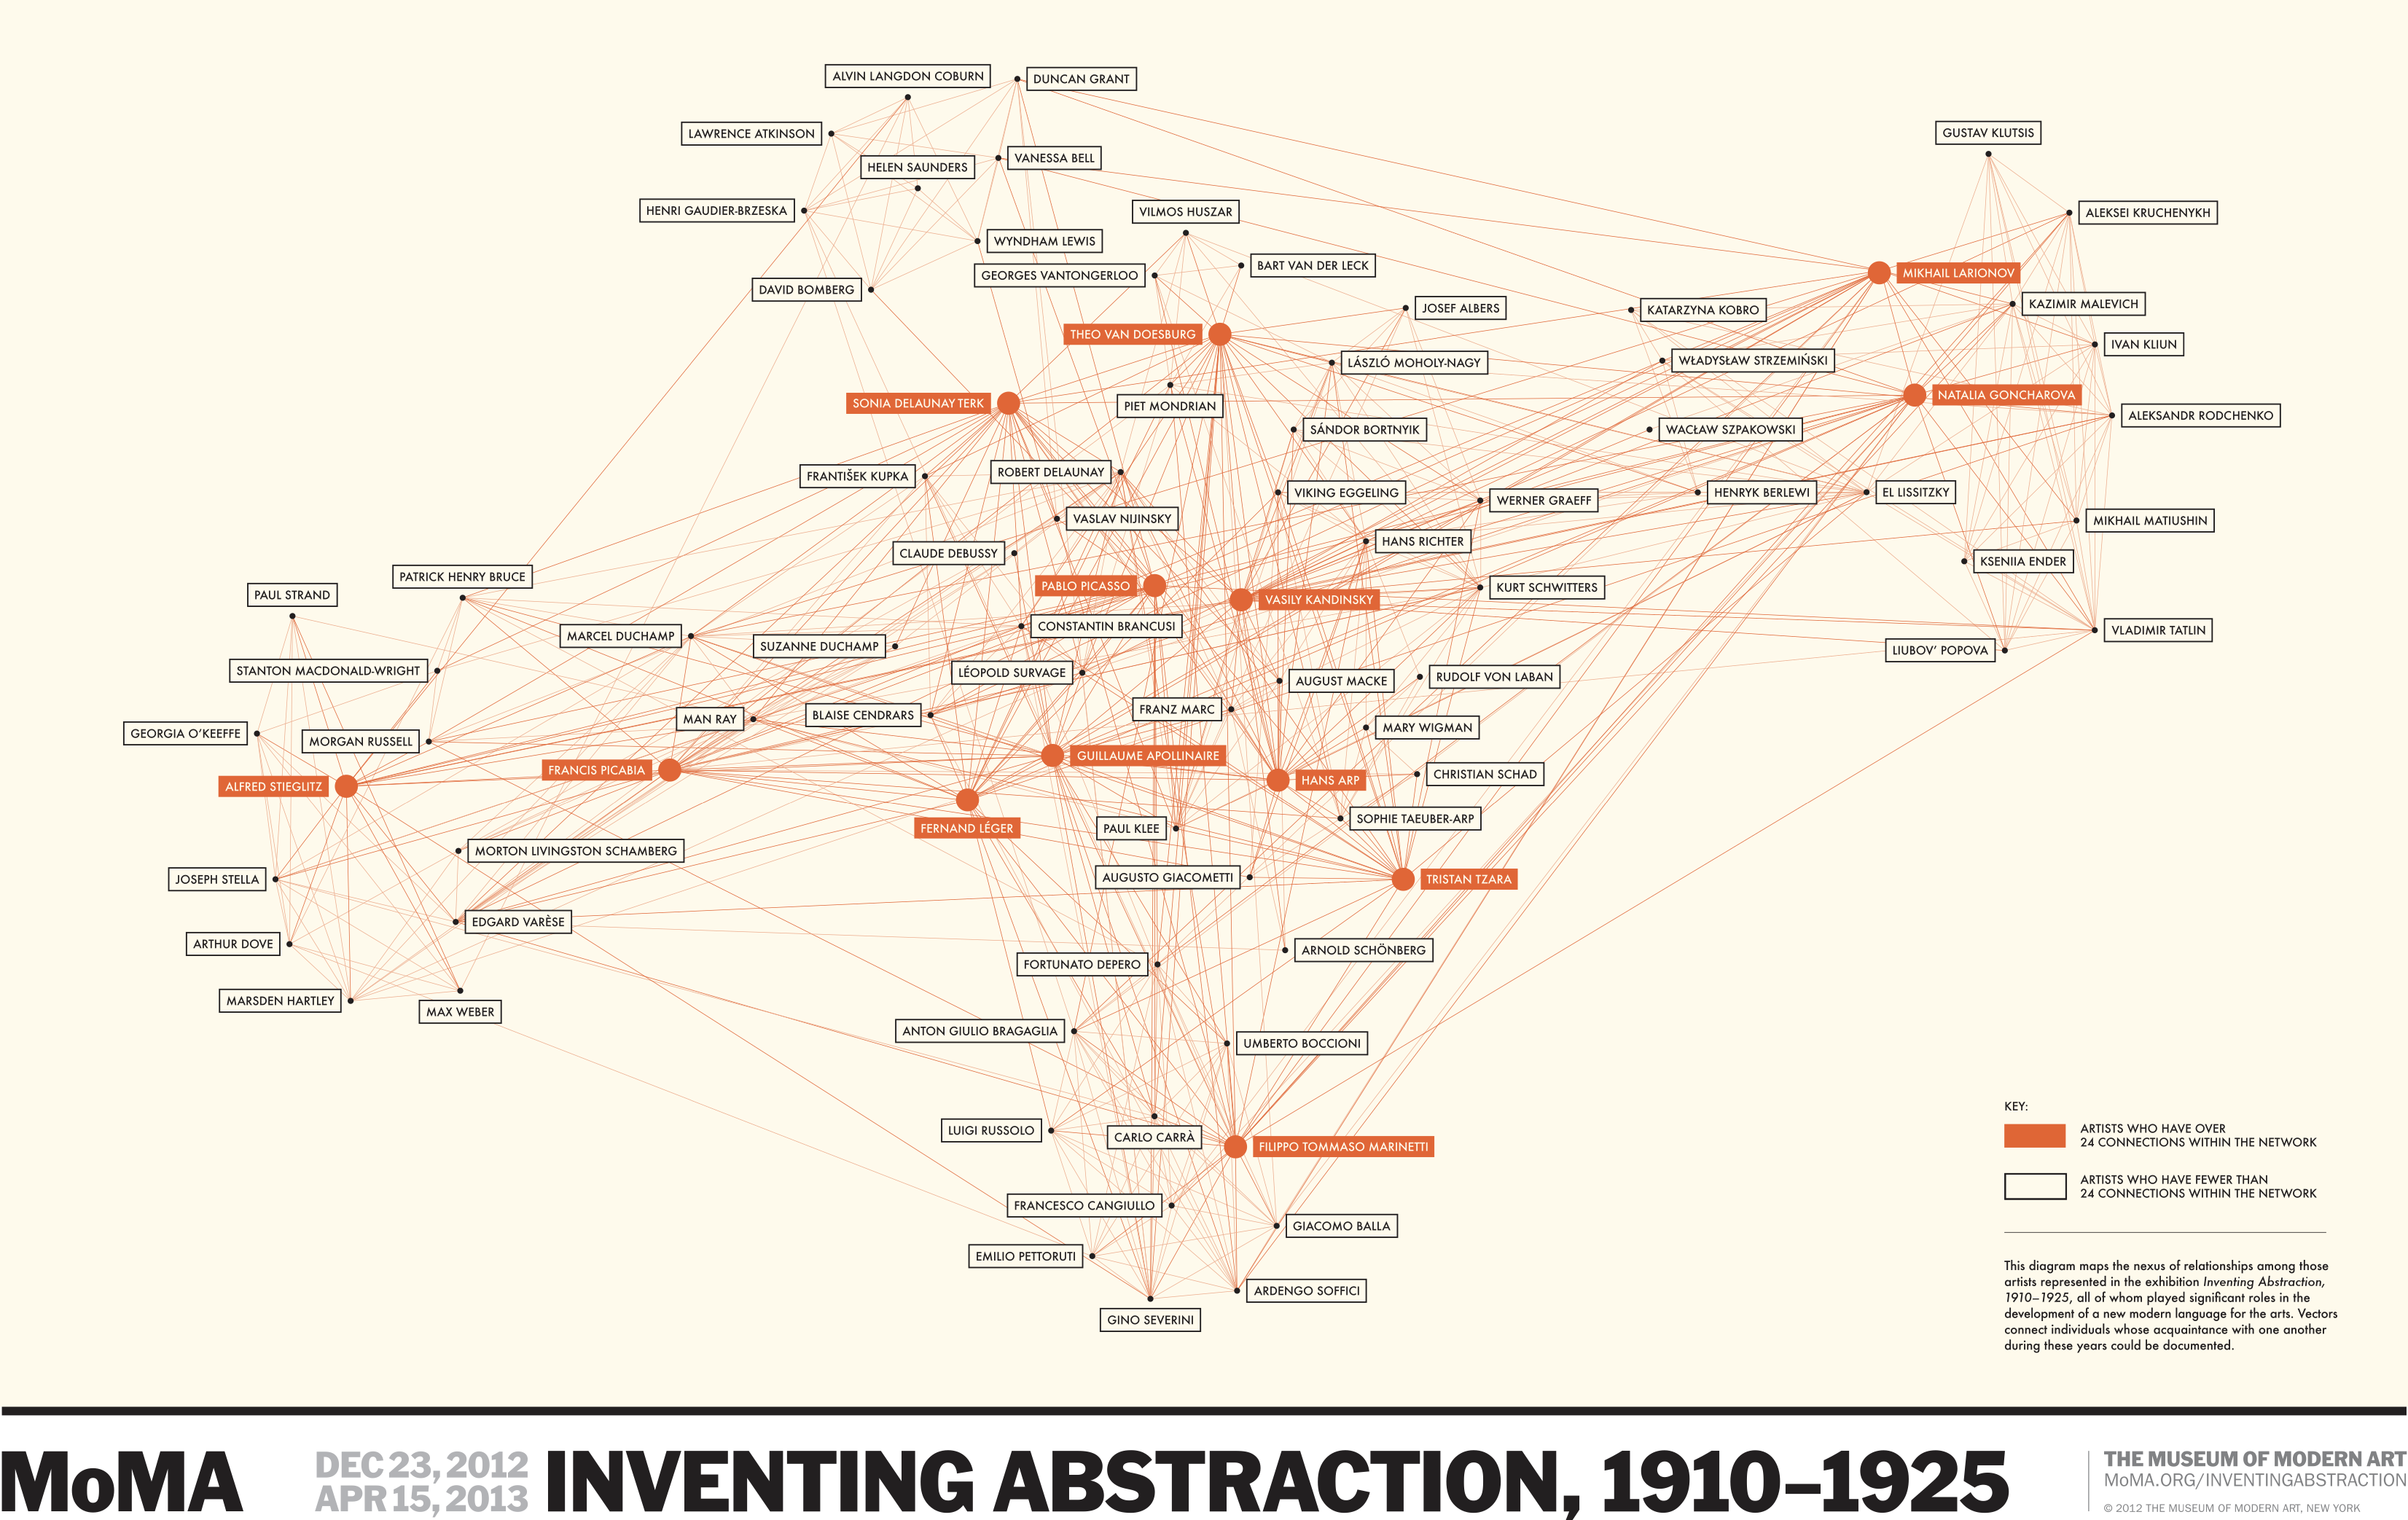
\includegraphics[width=\textwidth]{graphics/2-literature-review/26}
    \end{center}
    \caption{Inventing abstraction by MoMA}
    \label{fig:figure2.26}
\end{figure}

When speaking about the connections between artists, one example of it is presented in \Cref{fig:figure2.26}, the visualization by the
Museum of Modern Arts for the Inventing Abstraction exhibition~\citep{moma}. It is interactive and there is a possibility to click on any
artist in order to explore only their connections with others. Artists with their names in red are the ones with the most connections.

An example of the PolyCube framework (see \Cref{sec:data-visualization-cultural-heritage}) used in cultural heritage was the visualization
of the life and work of an amateur photographer Charles Weever Cushman~\citep{mayr2019visualizing}. Cushman’s work was presented using
geographic and categoric space-time cubes where each cube depicted a relevant pattern with the temporal development between 1938 and 1955.

\begin{figure}[hbt!]
    \centering
    \begin{subfigure}{.5\textwidth}
        \centering
        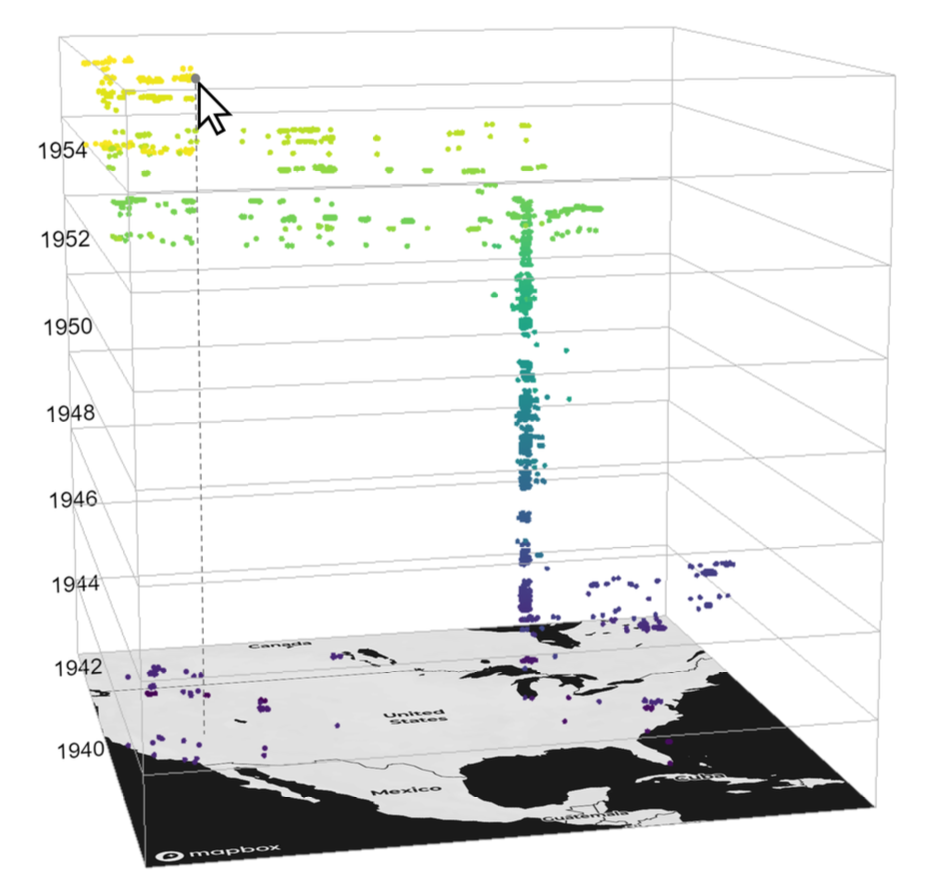
\includegraphics[width=0.9\linewidth]{graphics/2-literature-review/artist1}
    \end{subfigure}%
    \begin{subfigure}{.5\textwidth}
        \centering
        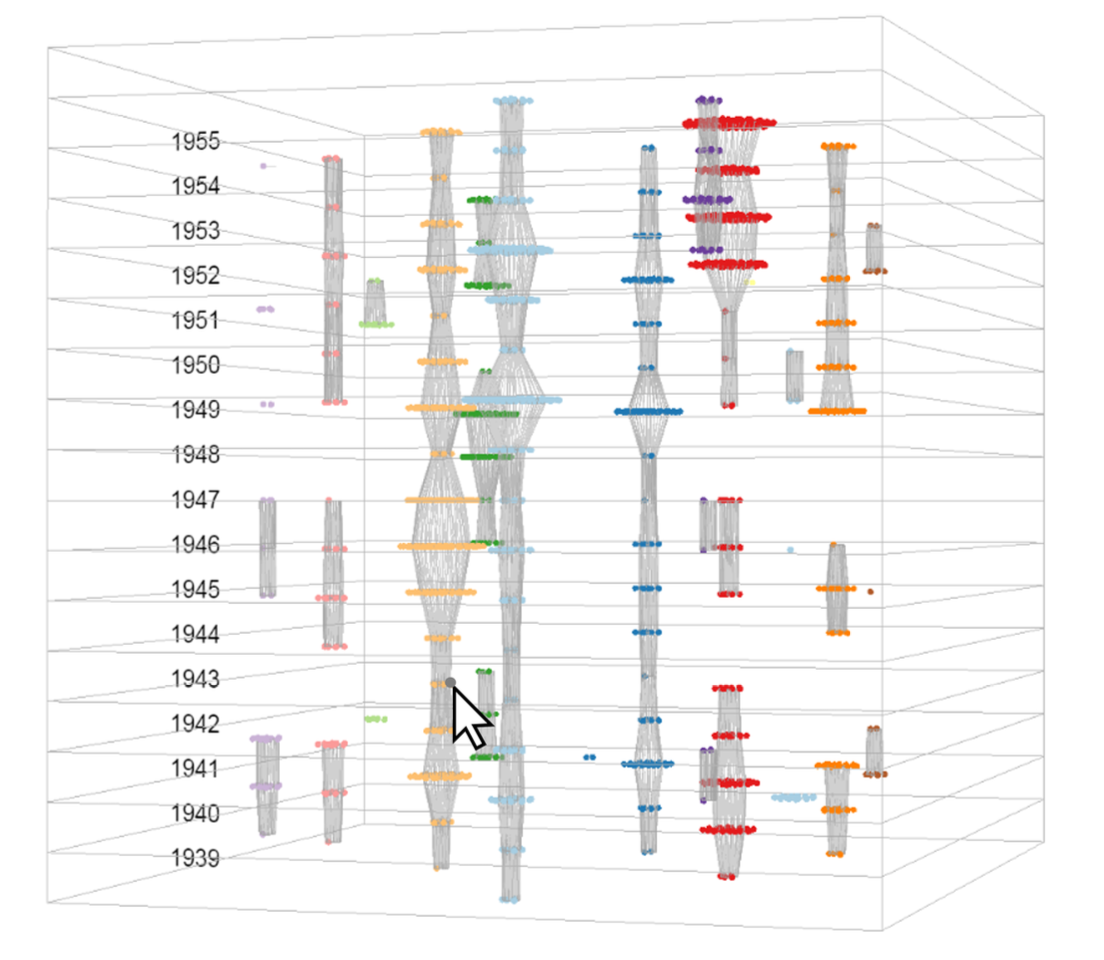
\includegraphics[width=\linewidth]{graphics/2-literature-review/artist2}
    \end{subfigure}
    \caption{Geographical (left) and categorical (right) space-time cube representations of Charles W. Cushman's life and  work}
    \label{fig:figure2.artist}
\end{figure}

The figure on the left shows the geographical pattern of the photographs where the earliest ones are colored in violet and the latest ones in
yellow. Scattered points mean the photographer was traveling extensively during that time. The figure on the right presents us with
categorical patterns based on the main photography genres. Each category was colored differently and dispersed among the timeline thus we can
examine the number of specific photograph genres taken every year. For example, in 1943 he took the least number of photos.

\clearpage

\begin{figure}[hbt!]
    \begin{center}
        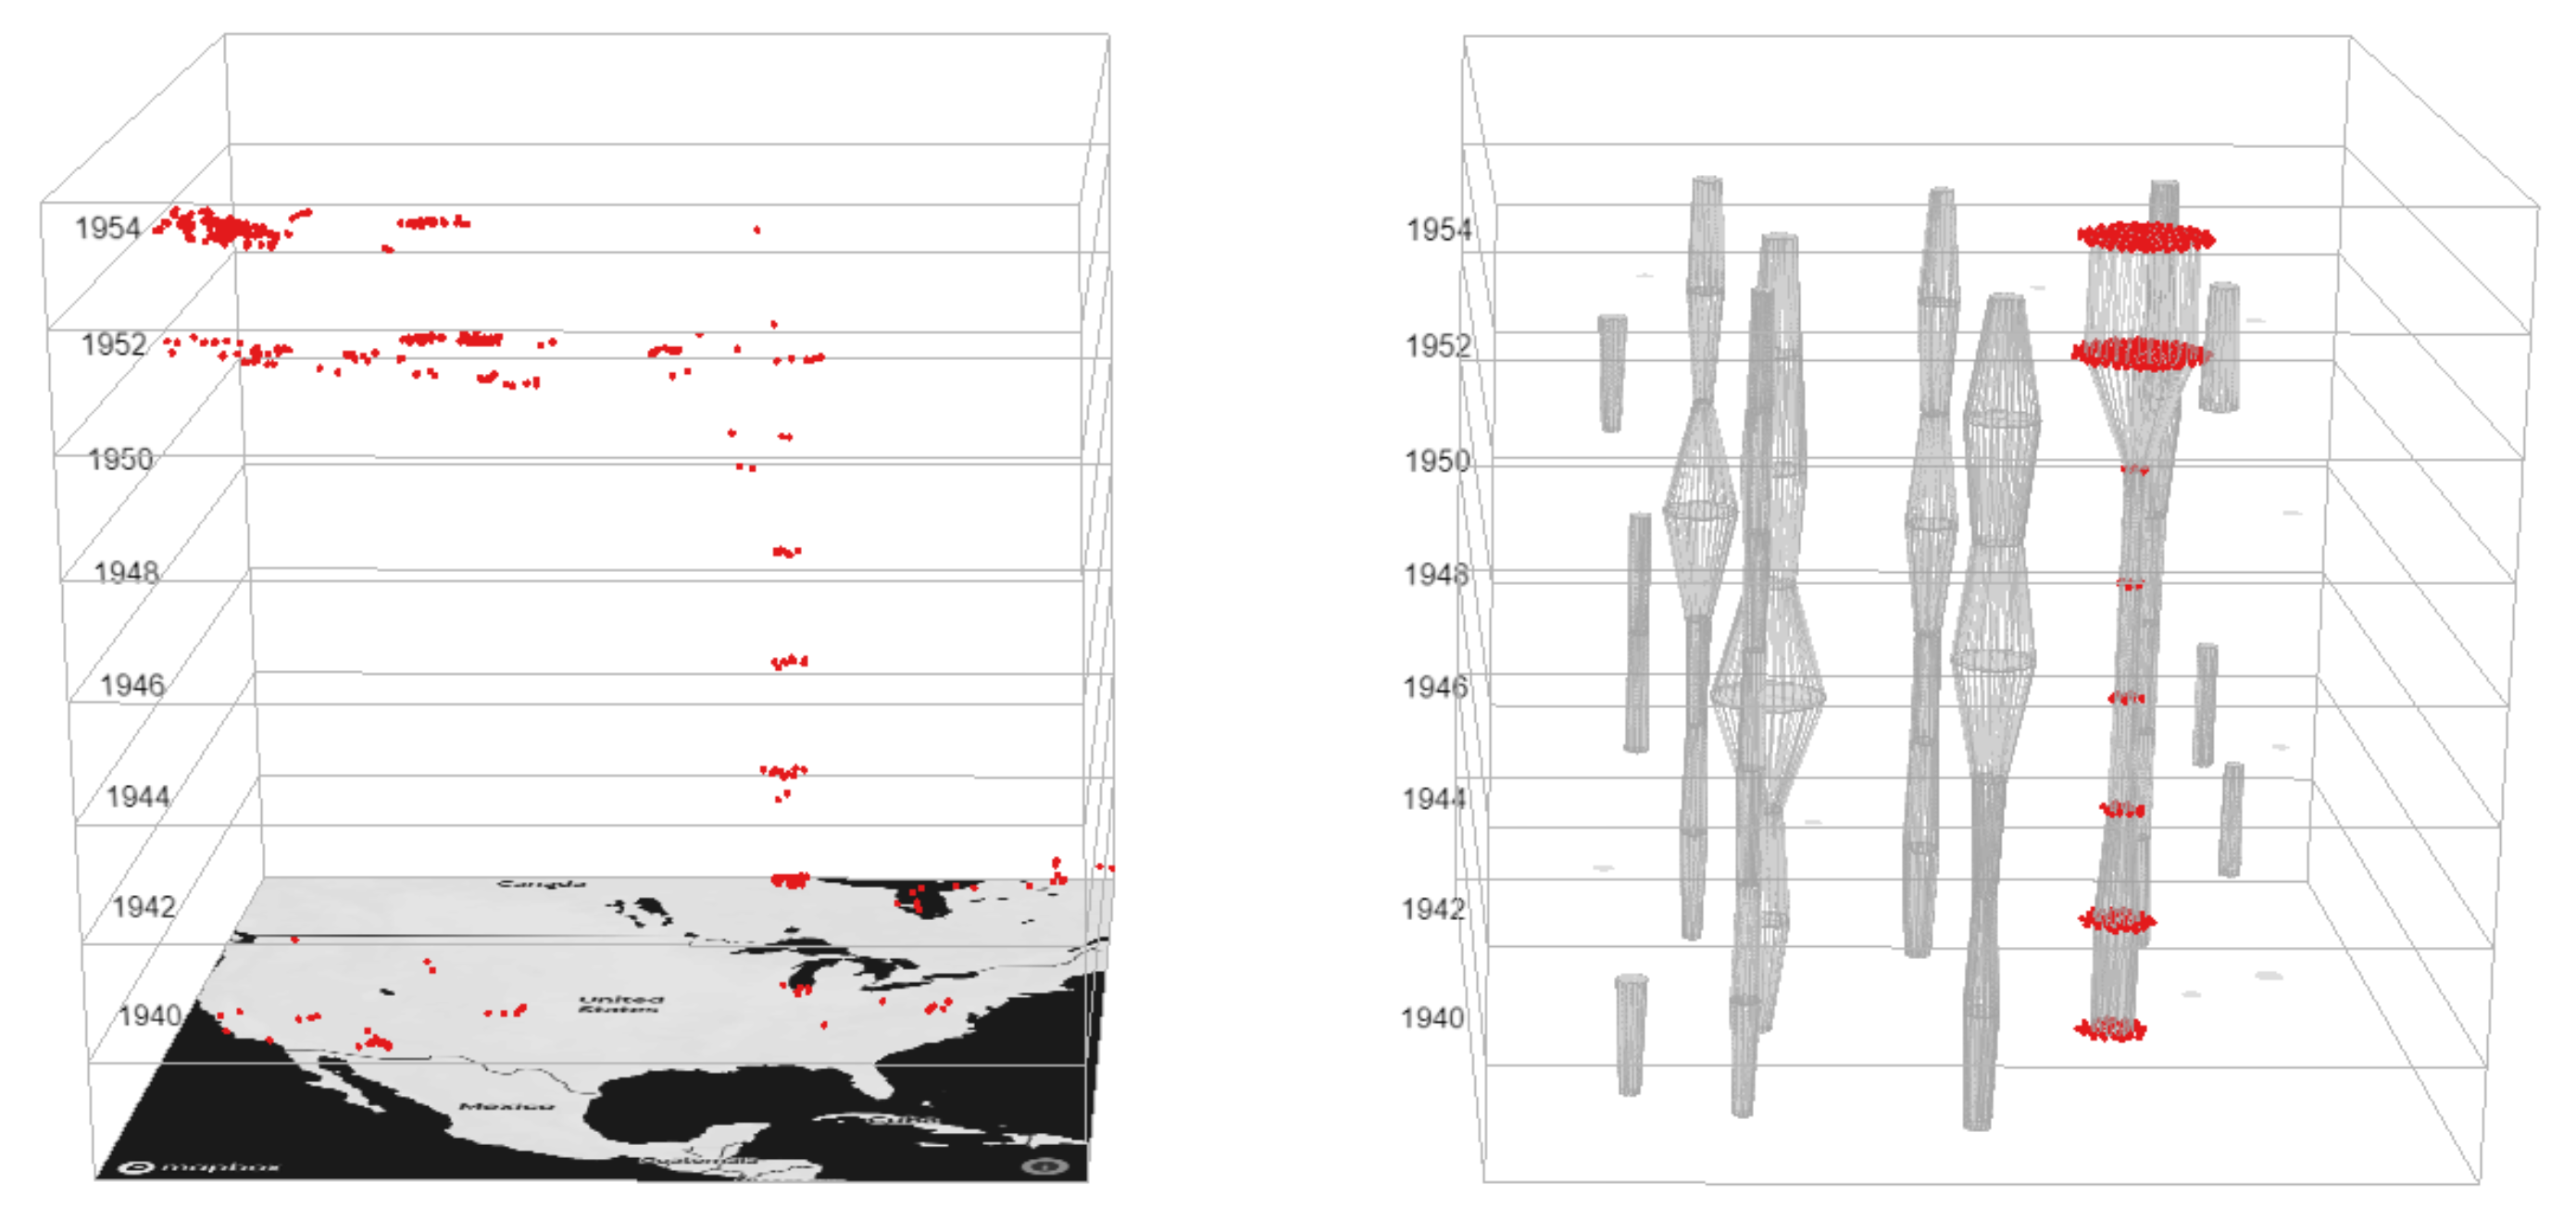
\includegraphics[width=\textwidth]{graphics/2-literature-review/artist3}
    \end{center}
    \caption{Landscape genre filtered space-time cube representations of Charles W. Cushman's work}
    \label{fig:figure3.artist}
\end{figure}

The paper also shows the framework providing us with the possibility to filter the genre and present a “coordinated multiple cubes” view. In
the figure above, we can see the filtered landscape photographs and explore their spatio-temporal distribution closely.
